\chapter{Implementation} \label{implementation}
This Chapter describes step by step how the prototype for malicious DoH traffic detection is implemented into SecGrid. First, Section \ref{pipeline} is an overview where the whole pipeline of the newly implemented prototype is shown. Section \ref{impl_clumping} describes the clumping process. In Section \ref{feat_extr_impl}, the feature extraction is depicted, whereas the computation of the statistical metrics and every feature type (header features, packet information features, and the new features) is exemplified in the respective Subsection, inclusively how they are saved. Section \ref{training_ds} presents the training data-sets that are later used by the ML models. First the preprocessing procedure is described, followed by the compilation of the training data-sets. Finally, in section \ref{ml_model} the centerpiece of this thesis is presented: two LGBM algorithms are trained to detect malicious DoH traffic within a two layered system. Subsequent to this Section, the hyper-parameter tuning of the two ML models is presented. 

\section{Pipeline} \label{pipeline}
The implementation of every component results in a fully working prototype for the detection of malicious DoH traffic. Figure \ref{fig:pipeline} shows the illustrated pipeline of this prototype. It takes a PCAP-file as input, which is handled like every other file in SecGrid according to Figure \ref{architecture}, i.e. it is forwarded by the RESTful-API, runs through the \textit{ddos\_dissector}, the \textit{converters}, and the \textit{Packet Decoder} until it arrives in the \textit{Protocol Parser}. The \textit{Protocol Parser} hands over every single flow to the \textit{TCP Tracker}, which extracts the packet information and collects the flow information and gives it back to to the \textit{Protocol Parser}. The protocol parser hands over every single flow to the \textit{Feature Extraction}, which computes all the feature values of the clumped flow, which is then saved into a CSV-file. This procedure is repeated until every flow contained in the input PCAP-file is analyzed, clumped and saved in the CSV-file. The CSV-file that contains all the clumps with the respective feature-values is then forwarded to the two-layered malicious DoH detection component. In Layer 1, the clumps are separated into DoH traffic and non-DoH traffic, whereas only the DoH traffic is forwarded to the second Layer. The second Layer checks if the DoH traffic is malicious or benign. If malicious traffic is found, it is saved into a CSV-file and forwarded to the \textit{File Storage} of SecGrid.

\begin{figure} [h]
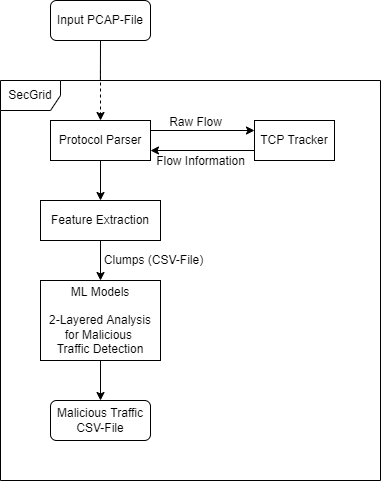
\includegraphics[scale=0.5]{images/pipeline.png}
\centering
\caption{Pipeline of the Data-Flow}
\label{fig:pipeline}
\end{figure}

\section{Clumping} \label{impl_clumping}
For the clumping process, as introduced in Section \ref{clumping}, the TCP-flows of the input files are separated and each flow builds one clump. Therefore, the parser of SecGrid in the file \textit{PcapParser.js} and the \textit{tcp\_tracker} of \textit{node-pcap} need to be adjusted, since the \textit{PcapParser.js} does not handle TCP flows so far and the \textit{tcp\_tracker} does not handle the packet size information in a useful way for this work and it does also not handle non-closing TCP flows. \textit{Node-pcap} is forked locally into the project as a folder such that it can be modified, before it was included as a dependency. 

So far, SecGrid used only the function of inspecting PCAP packets. \textit{node-pcap} is able to inspect complete TCP flows. Therefore, the parser is modified such that it collects every single TCP flow and as soon as the flow has ended, the parser emits the flow to the feature extraction, thus the ending flows are analyzed. Each flow has a property called \textit{state}, which is set to \textit{CLOSED} after the flow was closed by the \textit{tcp\_tracker} of \textit{node-pcap}. However, in a next step the non-ending flows have to be handled, since \textit{node-pcap} is able to handle packets with non ending flows, but they are not terminated and emitted to the feature extraction. Therefore the parser collects every flow in a JS object and every time a flow is returned closed, this flow is removed from the object. When the last packet is inspected by the \textit{tcp\_tracker}, the remaining flows in this object are all the flows which are non-ending. 

The parser goes through this list and calls the function \textit{forceClose} in the \textit{tcp\_tracker}. The \textit{tcp\_tracker} has to be adjusted such that it has this function \textit{forceClose}, which closes each open flow as soon as the last packet has passed through the parser and the flow is still open. The \textit{state} is set to \textit{OPEN} and the flow is emitted to the parser. After the parser called the \textit{forceClose} function and emitted the respective flow to the feature extraction, the flow is removed from the object. This process is repeated until the object is empty, meaning that all the flows of the PCAP file are handled and emitted to the feature extraction. 

The handling of non-ending flows is important since also non-ending flows can be affected by malicious influence. Since the \textit{tcp\_tracker} did not have a handling of such flows, it is crucial to implement it in this work because otherwise they would not have been further analyzed. Adding a new \textit{state } (\textit{OPEN}) aims to make the analysis even more precise compared to the related work, since there the aim of the flow-handling is mainly laid to the extraction of statistical properties. 

\section{Feature Extraction} \label{feat_extr_impl}
In this Section the Feature Extraction is presented in detail. It is included in the file \textit{MachineLearningFeatureExtractionDoH.js} as a subclass of the superclass \textit{AbstractPCAPAnalyser.js}. The flows handed over by the parser are analyzed here, whereas the flow is an object called "session", which contains the information of a single flow extracted by \textit{node-pcap}. The features of the "session" object used for the feature extraction of SecGrid are shown in Table \ref{tab:session}.

An important information to know about the \textit{tcp\_tracker} of \textit{node-pcap} is that it does not deliver all the information of a TCP packet. It delivers the information of the IPv4 layer and the TCP layer of every packet in the flow, but it ignores the frame information of the packet, i.e. in the case of the data-set \cite{CIRA-CIC-DoHBrw-2020} the \textit{Linux cooked-mode capture (SLL)}, which is a pseudo-protocol for capturing traffic with several devices at the same time \cite{sll}. Every packet contains this information, which has the size of 16 Bytes in most cases, in some very rare cases it can also be more. But this fact does not affect the quality of the data used negatively, since the data is a cleaner representation of TCP data without the SLL information. In that sense, the exclusion of such data improves the accuracy of the data.

\begin{center}
\begin{longtable}{ |l|l| }
\hline
Feature & Format \\
\hline
\textit{connect\_time} & \textit{float} (Time since 1970) \\
\hline
\textit{close\_time} & \textit{float} (Time since 1970) \\
\hline
\textit{src} & \textit{string}, "IP:Port", e.g. "192.168.20.111:44310" \\
\hline
\textit{dst} & \textit{string}, "IP:Port", e.g. "1.1.1.1:433" \\
\hline
\textit{send\_bytes\_ip} & \textit{int} \\
\hline
\textit{send\_bytes\_payload} & \textit{int}  \\
\hline
\textit{send\_bytes\_tcp} & \textit{int} \\
\hline
\textit{recv\_bytes\_ip} & \textit{int} \\
\hline
\textit{recv\_bytes\_payload} & \textit{int} \\
\hline
\textit{revc\_bytes\_tcp} & \textit{int} \\
\hline
\textit{send\_acks} & \textit{Object}, Object\{"ACK No.":"sending time"\} \\
\hline
\textit{recv\_acks} & \textit{Object}, Object\{"ACK No.":"receiving time"\} \\
\hline
\textit{send\_packets} & \textit{Object}, Object\{["Seq. No. + Data Length"]:"sending time"\} \\
\hline
\textit{recv\_packets} & \textit{Object}, Object\{["Seq. No. + Data Length"]:"receiving time"\} \\
\hline
\textit{send\_retrans} & \textit{Object}, Object\{["Seq. No. + Data Length"]:"sending time"\} \\
\hline
\textit{recv\_retrans} & \textit{Object}, Object\{["Seq. No. + Packet Length"]:"sending time"\} \\
\hline
\textit{state} & \textit{boolean} \\
\hline
\textit{total\_packet\_length} & \textit{array}, ["Packet Length"] \\
\hline
\caption{Features of the Session Object forwarded by the \textit{tcp\_tacker} and used for the Feature Extraction}
\label{tab:session}
\end{longtable}
\end{center}

Before extracting the features, a simple and short process is used to verify that only HTTPS traffic is analyzed, namely by checking if the source port or the destination port of the flow is port 433. With this procedure redundant traffic is filtered and not used for further analysis, which saves a lot of time for the actual analysis of HTTPS traffic, since this process can be time consuming enough depending on the size of the input PCAP file to be analyzed.

\subsection{Header Features}
The header features are extracted according to Section \ref{head_feat}. To extract the \textit{Source IP} and the \textit{Source Port}, the feature \textit{src} of the "session" object are used. For those two types, the functions \textit{getIP} and \textit{getPort} are implemented. \textit{getIP} returns the characters before the colon in \textit{session.src} or \textit{session.dst} to get the \textit{Source IP} or the \textit{Destination IP}, respectively. The function \textit{getPort} returns the numbers following the colon in the colon in \textit{session.src} or \textit{session.dst} to get the \textit{Source Port} or the \textit{Destination Port}, respectively. The extraction of the features \textit{Destination IP} and \textit{Destination Port} is identical to the extraction of \textit{Source IP} and the \textit{Source Port}, except that instead of \textit{src}, \textit{dst} is used. The feature \textit{Duration} is extracted by computing the delta of \textit{close\_time} and \textit{connect\_time} of the object "session".

To extract the feature \textit{Flow Bytes Sent}, the features \textit{send\_bytes\_ip}, \textit{send\_bytes\_payload}, and {send\_bytes\_tcp} are summed. \textit{send\_bytes\_ip} is the sum of IP information (the size of the payload and the header) of the IPv4 layer of every packet in the flow, \textit{send\_bytes\_payload} is the sum of the payload of the TCP layer of every packet in the flow, and {send\_bytes\_tcp} the header information (the size of the header) of the TCP layer in every packet in the flow. The feature \textit{Flow Bytes Received} is computed similar to the feature \textit{Flow Bytes Sent}, except that the features \textit{recv\_bytes\_ip}, \textit{recv\_bytes\_payload}, and {recv\_bytes\_tcp} are summed.

The extraction of the features \textit{Flow Sent Rate} and \textit{Flow Received Rate} is more complex. They require to first extract all the the times of outgoing and incoming packets. Therefore, all the values in the objects \textit{send\_acks} and \textit{send\_packets} are extracted and pushed into an array whenever a packet was sent. From this array, the maximum value and the minimum value is taken and the delta of those two values is computed and returned as \textit{Duration Sent}. For this process, the function \textit{getDurationSending} was implemented. In a second step the actual rate is computed by dividing the feature \textit{Flow Bytes Sent} which was beforehand computed by the \textit{Duration Sent}. This process was implemented in the function \textit{computeRate}. The feature \textit{Flow Sent Rate} is computed similarly, except that the function \textit{getDurationReceiving} uses the objects \textit{recv\_acks} and \textit{recv\_packets} and the function \textit{computeRate} divides \textit{Flow Received Rate} by \textit{Duration Received}.

\subsection{Statistical Metrics} \label{stat_met_impl}
The statistical features are computed according to the Section \ref{stat_met}. Every metric (see Table \ref{tab:impl_stat_met}) has its own function and the functions are designed to compute the metric of an array (here called "packets"). Thus the function for every metric has only to be implemented once and still the metrics for the \textit{Packet Length}, the \textit{Packet Time}, and the \textit{Packet Response} and \textit{Request Time} can be computed by using the metric functions. To avoid errors caused by empty arrays, each function checks first that the input array is not empty and then it computes the metric. If the input array is empty, it returns 0 instead. The metrics \textit{Mean}, \textit{Median}, \textit{Mode}, \textit{Variance}, and \textit{Standard Deviation} are all computed by using the respective function of the \textit{mathjs API} \cite{mathjs}. The functions \textit{Coefficient of Variation}, \textit{computeSkewFromMode}, and \textit{computeSkewFromMedian} are computed according to the Section \ref{stat_met} and are also using functions of \textit{mathjs} where needed.

\begin{center}
\begin{tabular}{ |l|l|l| }
\hline
Metric & \textit{Function\_Name(Input\_Array)} & Output Format\\
\hline
Mean & \textit{computeMean(packets)} & \textit{float} \\
\hline
Median & \textit{computeMedian(packets)} & \textit{float} \\
\hline
Mode & \textit{computeMode(packets)} & \textit{int} \\
\hline
Variance & \textit{computeVariance(packets)} & \textit{float} \\
\hline
Standard Deviation & \textit{computeStandardDeviation(packets)} & \textit{float} \\
\hline
Coefficient of Variation & \textit{computeCoefficientOfVariation(packets)} & \textit{float} \\
\hline
Skew from Mode & \textit{computeSkewFromMode(packets)} & \textit{float} \\
\hline
Skew from Median & \textit{computeSkewFromMode(packets)} & \textit{float} \\
\hline
\end{tabular}
\captionof{table}{Function Names of the Statistical Metrics}
\label{tab:impl_stat_met}
\end{center}

\subsection{Packet Information Features}
The packet information, which include the information of the packet size, packet time and the response- and request time, features are computed using the metric computation functions presented in the previous Section \ref{stat_met_impl}. The \textit{Input\_Array} for the packet length features is the feature \textit{total\_packet\_length} of the object "session". This feature is the output of a retroactively implemented process into \textit{node-pcap}. This process is implemented in this thesis since \textit{node-pcap} does not offer a feature which contains the packet length of every packet. The output is an array that contains the summed features \textit{send\_bytes\_ip}, \textit{send\_bytes\_payload}, and {send\_bytes\_tcp} of every packet that was inspected by \textit{node-pcap}. The input array of the packet time features is extracted by the function \textit{getTotalTimes}, which pushes every timestamp contained in the objects \textit{send\_packets}, \textit{recv\_packets}, \textit{send\_acks}, and \textit{recv\_acks} into one array, sorts the array, subtracts the smallest timestamp from every timestamp in this array and returns the array.  

The input array of the packet response- and request time features is computed with multiple functions. The functions \textit{getTimesSent(session)} and \textit{getTimesReceived(session)} both receive the session object as the input. \textit{getTimesSent(session)} extracts the values of the features \textit{send\_packets} and \textit{send\_acks} of the "session" object, pushes them into an array and returns a sorted array with all the timestamps when packets or TCP segments that have an ACK flag (ACKs) were sent. \textit{getTimesReceived(session)} is similar, but it returns a sorted array with the timestamps when packets or ACKs were received by extracting them from the features \textit{recv\_packets} and \textit{recv\_acks} of the object "session". Finally, the differences are computed by the function \textit{getRequRespDifference} which takes the two sorted arrays of timestamps of sent and received packets as input and computes the time differences between outgoing and incoming packet timestamps at the client's side according to Algorithm \ref{alg:reqResp}.

\begin{center}
\begin{algorithm}
\caption{Compute the Difference between outgoing and incoming Timestamps}
\begin{algorithmic}
\Require $timesSentSorted, timesReceivedSorted$
\Ensure $timesSentSorted.length \neq 0, timesReceivedSorted.length \neq 0$
\State $n \leftarrow timesSentSorted.length$
\State $m \leftarrow timesSentReceived.length$
\State $requestResponseDifference \leftarrow []$
\For{$i=0..n$}
\For{$j=1..m$}
\If{
\begin{varwidth}
$timesReceivedSorted[j] > timesSentSorted[i] \land $ \par
\hskip\algorithmicindent $ timesReceivedSorted[j] < timesSentSorted[i+1]$
\end{varwidth}
}
\State $difference = timesReceivedSorted[j] - timesSentSorted[i]$
\State $requestResponseDifference.next \leftarrow difference$
\end{algorithmic}
\label{alg:reqResp}
\end{algorithm}
\end{center}

\subsection{Novel Features}
The novel features proposed by in this thesis are extracted according to Section \ref{new_feat}. The state is computed with the function \textit{getState(session.state)}, which takes the session state as input and returns 1 if it is \textit{CLOSED}, if it is \textit{OPEN} it returns 0. The values 1 and 0 are chosen since the LGBM algorithm is is not able to handle the string values \textit{OPEN} and \textit{CLOSED}. The \textit{Number of Application Packets Sent} is the length of the object \textit{send\_packets} and the \textit{Number of Application Packets Received} is the length of the object \textit{recv\_packets}. The extraction of the \textit{Number of ACKs Sent} and \textit{Number of ACKs Received} is similar, since those two values are computed by takin the length of the object \textit{send\_acks} and \textit{recv\_acks}. Again, the extraction of \textit{nr\_retrans\_sent} and \textit{nr\_retrans\_reveived} is similar to the two latter pairs, it is the length of the objects \textit{send\_retrans} and \textit{recv\_retrans}, respectively. The \textit{Total Packet Length} is computed with the function \textit{getTotalPacketLength(session)}, which takes "session" as the input and sums up the values \textit{send\_bytes\_ip}, \textit{send\_bytes\_payload}, \textit{send\_bytes\_tcp}, \textit{recv\_bytes\_ip}, \textit{recv\_bytes\_payload}, and \textit{recv\_bytes\_tcp}.

\subsection{Saving Process}
The extracted features have to be persisted for the model training phase. This assignment is performed by the function \textit{createNewFlowData(session)}, which takes the "session" object as an input. Inside this function, all the needed values of the features are computed and stored into an object \textit{newPacketMiningData}, which is basically a list of all the features. This list is then returned by the function. The output of the function is then pushed into a global array called \textit{result}. After the analysis input PCAP file is finished, the \textit{result} array is written into a CSV file, which is then stored in the project for further usage.

\section{Training Data Sets} \label{training_ds}
With the feature extraction phase implemented as described in \ref{feat_extr_impl}, training data needs to be preprocessed as shown in this section. The two layered approach for detecting malicious traffic requires two data-sets with different content which are presented here. Thus, the data must first be extracted from the data-set \cite{CIRA-CIC-DoHBrw-2020} and bad data-points have to be removed. This step is described in the Section \ref{preprocessing}. After the preprocessing process, the training data-sets (TSL1 and TSL2) can finally be generated, these processes are described in the Sections \ref{tsl1} and \ref{tsl2}.

\subsection{Preprocessing} \label{preprocessing}
In a first step, the data has to be extracted from the data-set. The data-set is separated into two different directories, one for benign DoH and non-DoH traffic files and another one for malicious DoH traffic files. The directory with benign DoH and non-DoH traffic files is split into the two directories \textit{Chrome} and \textit{Firefox} which are the browser with whom the traffic data has been generated by \cite{montazerishatoori2020anomaly}. Both of these directories are again split into four different directories called \textit{AdGuard}, \textit{Cloudflare}, \textit{Google}, and \textit{Quad9} which are the DoH servers which have been addressed to generate the traffic data. The IP addresses of the DoH resolvers which were used are listed in Table \ref{tab:doh_ips}

\begin{center}
\begin{longtable}{ |c|c| }
\hline
\multicolumn{2}{|c|}{DoH Resolver IP-Address} \\
\hline
1.1.1.1 & 8.8.4.4 \\
\hline
8.8.8.8 & 9.9.9.9 \\
\hline
9.9.9.10 & 9.9.9.11 \\
\hline
176.103.130.131 & 176.103.130.130 \\
\hline
149.112.112.10 & 149.112.112.112 \\
\hline
104.16.248.249 & 104.16.249.249 \\
\hline
\caption{IP-Addresses of the DoH Servers used for the Data-Set \cite{CIRA-CIC-DoHBrw-2020}}
\end{longtable}
\label{tab:doh_ips}
\end{center}

With this list, it is possible to distinguish between DoH data and non-DoH data in the data-set. In a further step, every folder is analyzed separately and the data is saved in a separate CSV file. The features are ordered according to the order which was presented in Section \ref{feature_extraction_design}. In addition to those features, two further features are added, one called \textit{doh} which is set to 1 if the data is DoH traffic or 0 if it is non-DoH traffic, the other is called \textit{malicious} and receives the value 1 if it is malicous traffic or 0 if it is benign traffic. Since every folder contains many files and not every file can be analyzed by handing them separately, the script \textit{analyze.sh} is written. This is a Unix-Shell script that basically steps through every file of the folder and executes the Feature Extraction process of SecGrid. Table \ref{tab:benign_doh} and Figure \ref{fig:benign_doh} show how many flows of each kind have been extracted from the respective directories after deleting the lines whose feature values are zero. These zero-lines are unusable and would only distort the ML model.

\begin{center}
\begin{longtable}{ |l|c|c|c|c| }
\hline
 & AdGuard & Cloudflare & Google & Quad9 \\
\hline
Chrome (DoH) & 51 & 90 & 196 & 1968 \\
Firefox (DoH) & 13'513 & 1670 & 2678 & 10'089 \\
\hline
Chrome (non-DoH) & 27'729 & 50'152 & 50'512 & 104'044 \\
Firefox (non-DoH) & 66'864 & 112'376 & 70'272 & 123'107 \\
\hline
\caption{Number of total extracted benign DoH and Non-Doh Flows}
\end{longtable}
\label{tab:benign_doh}
\end{center}

\begin{figure}[h]
\caption{Totally Extracted Flows (DoH and non-DoH)}
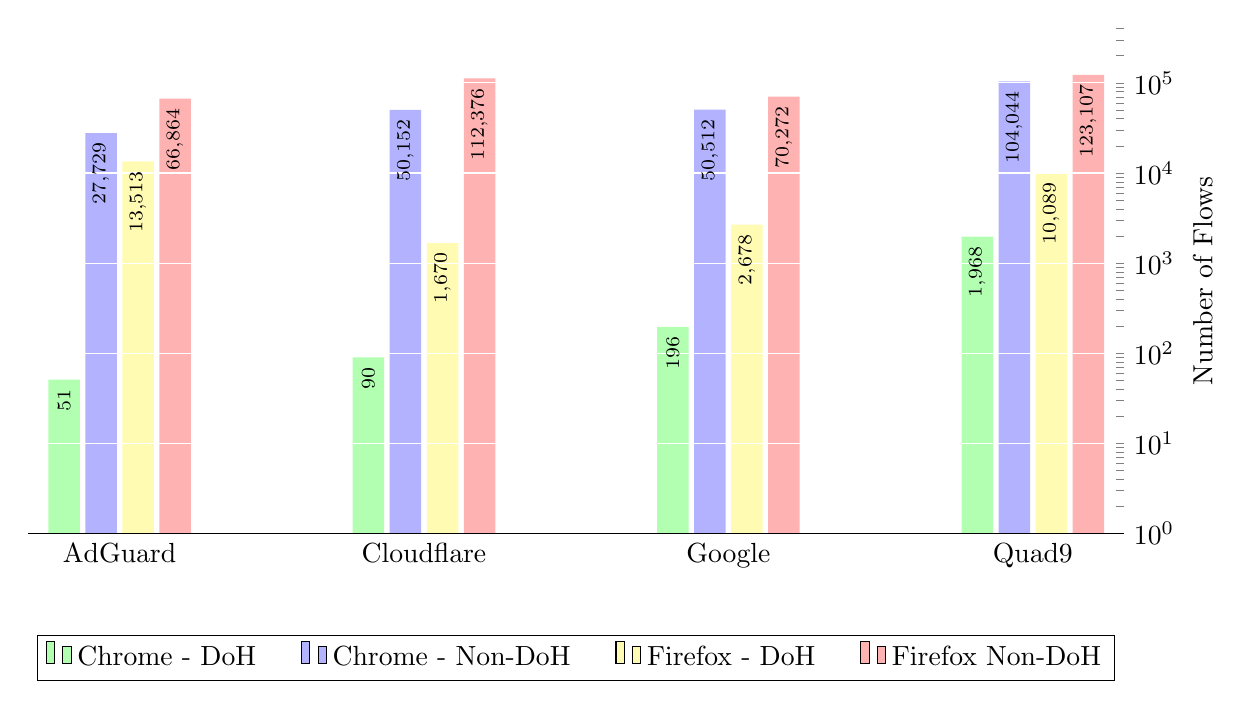
\begin{tikzpicture}
  \centering
  \begin{axis}[
        ybar, axis on top,
        title={},
        height=8cm, width=15.5cm,
        bar width=0.4cm,
        ymajorgrids, tick align=inside,
        major grid style={draw=white},
        enlarge y limits={value=.1,upper},
        ymin=1, ymax=125000,
        axis x line*=bottom,
        axis y line*=right,
        y axis line style={opacity=0},
        ymode = log,
        tickwidth=0pt,
        enlarge x limits=true,
        legend style={
            at={(0.5,-0.2)},
            anchor=north,
            legend columns=-1,
            /tikz/every even column/.append style={column sep=0.5cm}
        },
        ylabel={Number of Flows},
        symbolic x coords={
            AdGuard,
            Cloudflare,
            Google,
            Quad9
        },
       xtick=data,
       nodes near coords={
        \pgfmathprintnumber[precision=10]{\pgfplotspointmeta}
       },
       point meta=rawy,
       nodes near coords style={
            /pgf/number format/fixed,
            /pgf/number format/precision=5
            anchor=east,
            rotate=90,
            font=\scriptsize,
            left,
            #1}
    ]
    \addplot [draw=none, fill=green!30] coordinates {
      (AdGuard,51)
      (Cloudflare, 90) 
      (Google,196)
      (Quad9,1968) };
    \addplot [draw=none, fill=blue!30] coordinates {
      (AdGuard,27729) 
      (Cloudflare,50152)
      (Google,50512) 
      (Quad9,104044) };
   \addplot [draw=none,fill=yellow!30] coordinates {
      (AdGuard,13513)
      (Cloudflare, 1670) 
      (Google,2678)
      (Quad9,10089) };
    \addplot [draw=none,fill=red!30] coordinates {
      (AdGuard,66864) 
      (Cloudflare,112376)
      (Google,70272) 
      (Quad9,123107) };
   

    \legend{Chrome - DoH, Chrome - Non-DoH, Firefox - DoH, Firefox Non-DoH}
\end{axis}
\label{fig:benign_doh}
\end{tikzpicture}
\end{figure}

The directory with malicious DoH traffic files is split into three different folders, \textit{DNS2TCP}, \textit{DNScat2}, and \textit{iodine}, which are the tunnel tools which are used to generate the malicious traffic data. Since TSL1 will contain also some flows of malicious DoH data, the data in these directories must also be analyzed, the \textit{doh} feature is set to 1. Table \ref{tab:malicious_doh} indicates how many flows per tunnel tool were extracted, again after removing the lines with blank cells to avoid a distortion of the ML model.

\begin{center}
\begin{longtable}{ |l|c|c|c| }
\hline
DoH Malicious & \textit{DNS2TCP} & \textit{DNScat2} & \textit{iodine} \\
\hline
No. of Flows & 121'508 & 10'289 & 12'352 \\
\hline
\caption{Number of total extracted malicious DoH Flows}
\end{longtable}
\label{tab:malicious_doh}
\end{center}

For the second layer the benign and the malicious traffic data must be analyzed again. This time the features will be ordered according to the order for the second layer in Section \ref{training_ds}. The additional feature which is an indicator for benign or malicious traffic is this time called \textit{malicious} and set to 1 if the traffic is malicious, if t is benign it is set to 0.

Since the analysis of the PCAP-files in the data-set in each case was exported to a CSV-file, the deletion of zero-values was feasible. Excel has the function to split text in columns, the splits are always made when a comma (",") was set. Then the columns \textit{flow\_sent\_rate}, \textit{packet\_length\_median}, \textit{packet\_time\_median}, and \textit{response\_request\_median} are filtered with the respective function in Excel. The column \textit{flow\_sent\_rate} is chosen, since there it is an indicator for empty packet length arrays, the columns \textit{flow\_sent\_rate}, \textit{packet\_length\_median}, \textit{packet\_time\_median}, and \textit{response\_request\_median} are chosen since they are also indicators for empty arrays that were parsed. With this filter, it is possible to look for cells that contained zero values. The respective rows are deleted such that the finished table contains as few zero values as possible. The file is reset onto the format it had before by adding the columns together, separated with commas, such that it is possible to further process them.

\subsection{Training Data Set of Layer 1} \label{tsl1}
The composition of the Training Data Set of Layer 1 (TSL1) must be chosen in a way such that the ML model of Layer 1 is able to distinguish between DoH traffic and non-DoH traffic. In Section \ref{training_ds} the total amount of 40'00 data-points is determined. Therefore, the ratio of DoH traffic and non-DoH traffic in the training data-set is set to have an equal distribution of both types. Important here is that all the features that were computed are pushed and saved into TSL1. 

For the non-DoH data, the equal amount of 2500 data-points from every file listed in Table \ref{tab:benign_doh} is taken. This makes a total amount of 20'000 data-points of non-DoH traffic. To make sure that the data-points are as various as possible, the data-points are chosen randomly with the function \textit{sample()} that can be used for dataframes and which is taken from the Pandas library \cite{pandas} in Python. The data-points are then written into a CSV-file called \textit{TSL1.csv}.

The composition of the DoH data part of TSL1 is more complex, since especially the DoH traffic that was collected with Chrome is very sparse. Therefore, the distribution of the DoH traffic is chosen to be one half (10'000 data-points) benign and the other half malicious DoH traffic. From  each of then benign DoH traffic data-sets which were gathered using Chrome, half of the available data was used for TSL1, which results in 1160 data-points. The remaining 8840 data-points are taken from the benign DoH traffic data-sets which were gathered using Firefox. The part with the malicious DoH traffic is easier to compose, since there are enough data-points available. From the data-set that was generated using the \textit{DNS2TCP} tunnel tool, the amount of chosen data-points is 4000, since it is the largest data-set. The amount chosen from the \textit{DNScat2} and \textit{iodine} data-sets was 3000 each. For both parts of the DoH traffic data, the data-points are chosen randomly, again using the function \textit{sample()} of Pandas. Table \ref{tab:tsl1} shows the distribution of the data-points that were chosen for \textit{TSL1.csv}.

\begin{center}
\begin{longtable}{ |l|l|c|c|c|c| }
\hline
\multicolumn{2}{|c|}{ } & \makecell{Non-DoH\\(Chrome)} & \makecell{Non-DoH\\(Firefox)} & \makecell{DoH\\(Chrome)} & \makecell{DoH\\(Forefox)} \\
\hline
\multirow{4}{*}{Benign}
& AdGuard & 2500 & 2500 & 25 & 3500 \\
& Cloudflare & 2500 & 2500 & 45 & 800 \\
& Google & 2500 & 2500 & 90 & 1300 \\
& Quad9 & 2500 & 2500 & 1000 & 3240  \\
\hline
\multirow{3}{*}{Malicious}
& DNS2TCP & \multicolumn{2}{|c|}{0} & \multicolumn{2}{|c|}{4000}  \\
& DNScat2 & \multicolumn{2}{|c|}{0} & \multicolumn{2}{|c|}{3000} \\
& iodine & \multicolumn{2}{|c|}{0} & \multicolumn{2}{|c|}{3000} \\
\hline
\multicolumn{2}{|l|}{Total} & \multicolumn{2}{|c|}{20'000} & \multicolumn{2}{|c|}{20'000} \\
\hline
\caption{Distribution of the Data-Points in TSL1}
\label{tab:tsl1}
\end{longtable}
\end{center}

\subsection{Training Data Set of Layer 2} \label{tsl2}
The composition of the Training Data Set of Layer 2 (TSL2) must be chosen in a way such that the ML model of Layer 2 is able to distinguish between benign and malicious DoH traffic. The total amount of data is set to 40'000 data-points according to Section \ref{training_ds}. The ratio of the two types of traffic is set to have an equal distribution between the two types. Since TSL1 also contains benign and malicious traffic data, it is made sure that different data-points are used. Important here is also that all the features that were computed are given into TSL2. TSL2 is saved into a CSV file called \textit{TSL2.csv}.

The composition of the benign traffic data is complex, as already stated in Section \ref{tsl1}, since the data is sparse, especially the traffic that was gathered using the Google Chrome browser. Therefore, the other half of the available data is chosen from each of the files, which results in 1060 data-points. The remaining 18'840 data-points are taken from the benign DoH traffic data-sets which were gathered using Firefox. The composition of the malicious traffic is again easier due to the huge amount of available data. The amount of data gathered using the tunnel tool \textit{DNS2TCP} is chosen to be 8000 data-points, since it contains the most data, the amounts of data gathered using the tunnel tools \textit{DNScat2} and \textit{iodine} are chosen to be 6000 data-points each. Again, it was made sure that the data is chosen randomly by using the function \textit{sample()} of Pandas. Table \ref{tab:tsl2} shows the distribution of the data-points that were chosen for \textit{TSL2.csv}.

\begin{center}
\begin{longtable}{ |l|c|c|c| }
\hline
& \makecell{Benign\\(Chrome)} & \makecell{Benign\\(Firefox)} & Malicious \\
\hline
AdGuard & 25 & 10'000 & 0 \\
Cloudflare & 45 & 800 & 0 \\
Google & 90 & 1300 & 0 \\
Quad9 & 900 & 6840 & 0 \\
\hline
DNS2TCP & \multicolumn{2}{|c|}{0} & 8000 \\
DNScat2 & \multicolumn{2}{|c|}{0} & 6000 \\
iodine & \multicolumn{2}{|c|}{0} & 6000 \\
\hline
Total & \multicolumn{2}{|c|}{20'000} & 20'000 \\ 
\hline
\caption{Distribution of the Data-Points in TSL2}
\label{tab:tsl2}
\end{longtable}
\end{center}

\section{ML Model} \label{ml_model}
As introduced in Section \ref{LGBM}, Light Gradient Boosting Machine is chosen as the ML algorithm for both Layers. The whole pipeline is written in Python, since scikit-learn \cite{sklearn_api} is easy to apply, and it is an easily accessible API for ML algorithms. The LGBM-model is imported from \textit{ligthgbm} \cite{lightGBM}. To handle the data-sets, the Pandas library \cite{pandas} is used, the training data-set for Layer 1 is saved into a file called \textit{TSL1.csv}, the training data-set for Layer 2 is saved into a file called \textit{TSL2.csv}.

\subsection{Layer 1} \label{impl_l1}

\begin{figure} [h]
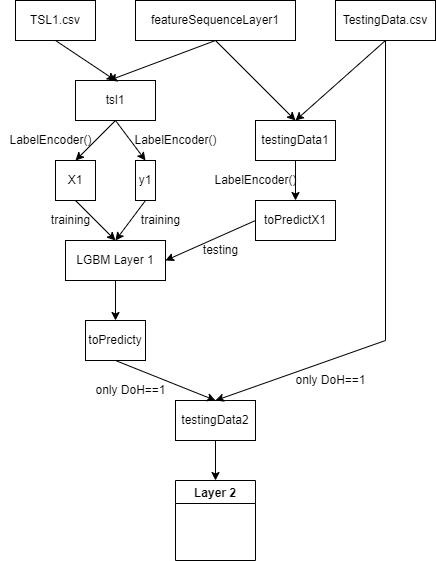
\includegraphics[scale=0.5]{images/layer_1.png}
\centering
\caption{Illustration of the Data Flow of Layer 1}
\label{fig:layer_1}
\end{figure}

The model of the first layer is trained with TSL1. To have the correct order of the features (according to \cite{BehnkeEtAl_FeatureEngineeringMLModelMaliciusDoHTraffic}), an array with the ordered feature names called \textit{featureSequenceLayer1} is defined, since \textit{TSL1.csv} does not have the correct feature-order yet. The first feature is \textit{doh}, which indicates whether the data-point is DoH traffic or not, as defined in Section \ref{preprocessing}. The file \textit{TSL1.csv} is read by using the function \textit{read\_csv} of Pandas and its content is saved in the dataframe \textit{trainingDataset1}. Subsequently, \textit{featureSequenceLayer1} is used to compose the data-set for Layer 1, i.e. every column of the feature that is contained in the sequence is added to the training dataframe called \textit{tsl1}.

Next, the matrix \textit{X1} which contains the values of all the features used to train the model, and the y1 vector which contains the labels to train the model are extracted and saved into the respective variable. Since LGBM is not able to handle float values, the next step is to convert the floats into integers, which is done using the \textit{LabelEncoder} of the \textit{sklearn} API. To make sure that LGBM is able to process every value, the flow values of X1 and y1 are transformed with the \textit{LabelEncoder}. Then the LGBM Classifier is initiated and trained with X1 and y1. The hyperparameters which are used are acquired in a Grid Search in Section \ref{hyp_par}. 

After the  model is trained, it is now able to predict the input data from the PCAP file to be tested. The file which contains the extracted features of the PCAP-file to be analyzed is loaded into a new dataframe called \textit{testingDataset1}. Again, the features need to be ordered using \textit{featureSequenceLayer1} to create the new dataframe \textit{toPredict1}. After iterating over \textit{testingDataset1} and extracting every feature-column needed, it is saved into the dataframe \textit{toPredict1}. Now the matrix \textit{toPredictX1}, containing all the feature values to be predcited, is extracted from the dataframe \textit{toPredict1}. Again, the \textit{LabelEncoder} ensures that the ML model is able to handle all the values contained in \textit{toPredictX1}. Then the matrix \textit{toPredictX1} is handed over to the LGBM model with the function \textit{classifierLayer1.predict(toPredictX1)}, which predicts the input data and gives back the vector \textit{toPredicty1}.

The resulting vector \textit{toPredicty1} contains the predictions of every clump extracted from the input PCAP file. The value on each line is either 0 or 1, with 0 meaning that the clump is non-DoH traffic data and 1 meaning that the clump is DoH traffic data. The vector \textit{toPredicty1} is then added to the dataframe \textit{testingDataset1} by creating a new column called \textit{DoH}. Subsequently, the data-points which have \textit{DoH} equal to 1 are extracted from \textit{testingDataset1} and saved into a new dataframe called \textit{testingDataset2}, which is the clumps classified as DoH traffic data. Finally, \textit{testingDataset2} is handed over to Layer 2, where it is further analyzed.

\subsection{Layer 2} \label{impl_l2}
The model of the second Layer is trained with TSL2, with the features ordered according to \cite{BehnkeEtAl_FeatureEngineeringMLModelMaliciusDoHTraffic} and the new features introduced in Section \ref{new_feat} appended directly afterwards. Before being able to start the training, the training data-set needs to be composed, since the input file \textit{TSL2.csv} does not have the correct feature order yet. The feature sequence is defined in the array \textit{featureSequenceLayer2} with the first feature \textit{malicious}, which indicates if the respective clump is malicious or benign traffic as defined in Section \ref{preprocessing}. The file is read by the function \textit{read\_csv()} of Pandas and saved into a pandas dataframe called \textit{trainingDataset2}. Subsequently, an iteration through the array \textit{featureSequenceLayer2} is conducted and every feature-name that is contained in this array is searched in the dataframe \textit{trainingDataset2} and the respective column is saved into a new dataframe called \textit{tsl2}.

The next step is to extract the X2 matrix and the y2 vector. X2 is the matrix which contains the training values for the ML algorithm, and y2 is the vector which contains the labels which are needed to classify the data. After these two Objects are extracted, the values have to be transformed into integer values, since LGBM is not able to handle float values. This is done by using the \textit{LabelEncoder}, according to the same procedure as in Layer 1. Finally, the data is prepared, and the ML model can be initiated and trained with X2 and y2. The hyperparameters which are used are acquired in a Grid Search in Section \ref{hyp_par}.

After the model is trained, it is ready to predict the input data which was handed over to \textit{testingDataset2} after the process of Layer 1. This data has already been separated from non-DoH traffic, thus the ML model of Layer 2 can now predict if the data is malicious or benign. Again, the data needs to be prepared by iterating over the array \textit{featureSequenceLayer2}, looking up the feature in the dataframe \textit{testingDataset2} and saving the respective column into the dataframe \textit{toPredict}, but this time the feature \textit{malicious} is left away. These values also need to be transformed into integer values by using the \textit{LabelEncoder}, since the data-set contains many features which have the format float. Now the feature values are extracted from the dataframe \textit{toPredict2} to construct the matrix \textit{toPredictX2} which contains the feature values for the prediction. Then, the matrix \textit{toPredictX2} is handed over to the LGBM model with the function \textit{classifierLayer2.predict(toPredictX2)}, which predicts the input data and gives back the vector \textit{toPredicty2} as the output. 

This output vector \textit{toPredicty2} contains the predictions of every data-point that was contained in the matrix \textit{toPredictX2}. The value on each line is either 0 or 1, whereas 0 means that the TCP-flow was benign DoH traffic and 1 means that the TCP-flow was malicious traffic. \textit{toPredicty2} is then added to the dataframe \textit{testingDataset2} with the feature name \textit{Malicious Traffic}. As a final step, the data-points that were predicted to be malicious are filtered from the \textit{testingDataset2} checking if there is a data-point which has the value 1 in the feature-column \textit{Malicious Traffic}. If there is a data-point that is malicious, it is extracted and stored in a CSV-file called \textit{maliciousTraffic.csv}. Figure \ref{fig:layer_2} illustrates the whole pipeline of Layer 2.

\begin{figure} [h]
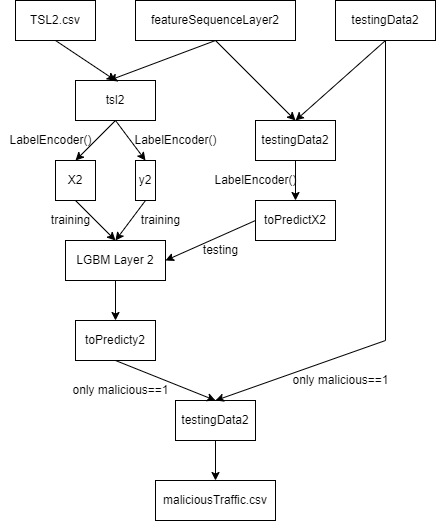
\includegraphics[scale=0.5]{images/layer_2.png}
\centering
\caption{Illustration of the Data Flow of of Layer 2}
\label{fig:layer_2}
\end{figure}

\subsection{Hyper-Parameter Tuning} \label{hyp_par}
According to the documentation of LGBM \cite{lightGBM}, the algorithm has three hyperparameters that are the most important to obtain good results and to avoid over-fitting of the model. Those three hyperparameters are \textit{num\_leaves}, \textit{min\_child\_samples}, and \textit{max\_depth}. Since the LGBM uses leaf-wise tree growth (see Figure \ref{fig:leaf_wise}) \textit{max\_depth} is the parameter to limit the tree depth and is set to -1 by default. \textit{num\_leaves} is the parameter that indicates how many leaves the model shall have and which controls how complex the model shall be. The number of leaves can be set to $num\_leaves = 2^{max\_depth}$ to have a symmetric tree model, but this should not be done because there is the risk of over-fitting the model. Therefore, the parameter \textit{num\_leaves} is chosen deliberately smaller than $2^{max\_depth}$. By default, it is set to 31 by scikit-learn. Finally, the parameter \textit{min\_child\_samples} indicates the number of data that is contained in a tree and depends on \textit{num\_leaves}. Small numbers can cause over-fitting, large numbers can cause under-fitting. \cite{lightGBM} states that setting this value to hundreds or thousands is enough, by default it is set to 20.

Furthermore, they mention the parameter \textit{max\_bin}, which indicates the maximum number of bins where the features will be bucketed, this means that LGBM packs continuous feature values into discrete bins. \textit{max\_bin} can be set between $0 < max\_bin <255$. They recommend trying the \textit{boosting\_type}, which is the way the model is boosted, set to \textit{dart}, by default it is set to \textit{gbdt}. Ultimately, the \textit{learning\_rate} which controls the number of trees that are grown in the training phase of the model. It is set to 0.1 b default.

\begin{figure} [h]
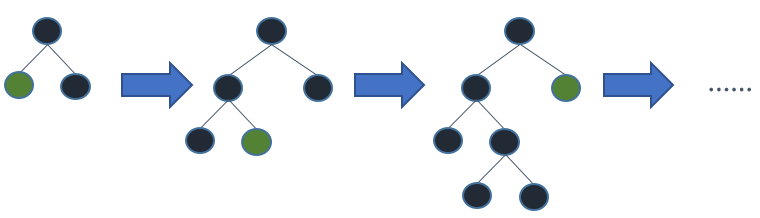
\includegraphics[scale=0.6]{images/leaf-wise.png}
\centering
\caption{Leaf-Wise Tree Growth \cite{lightGBM}}
\label{fig:leaf_wise}
\end{figure}

The setup for the Grid Search is as follows. The data is prepared like described in the Sections \ref{impl_l1} and \ref{impl_l2} and each time saved in the training matrix X containing the feature values and the training vector y containing the label values. Then, an array named \textit{tunedParameters} containing the the hyper-parameters to be tuned is implemented. Finally, the LGBM Classifier Algorithm is initiated together with the Grid Search, where the ML model and the and the array \textit{tunedParameters} are handed in as input. After the Grid Search, the model is trained with each combination of hyper-parameters to look for the best tuned parameters. The hyper-parameters are tuned in small batches to avoid long training times. The Following sections present the values that are used for the hyper-parameter optimization. After they are found, the hyper-parameters are adopted to the respective ML model.

\subsubsection{Layer 1}
The following snippet shows all the values that are tested with the Grid Search. Since totally 20 Grid Search are conducted using at most three values per parameter and also using at most three parameters at once, it is disclaimed to show all the experiments separately. Instead the list containing all the values that are used is shown.

\definecolor{bg}{gray}{0.95}
\DeclareTCBListing{mintedbox}{O{}m!O{}}{%
  breakable=true,
  listing engine=minted,
  listing only,
  minted language=#2,
  minted style=default,
  minted options={%
    linenos,
    gobble=0,
    breaklines=true,
    breakafter=,,
    fontsize=\small,
    numbersep=8pt,
    #1},
  boxsep=0pt,
  left skip=0pt,
  right skip=0pt,
  left=25pt,
  right=25pt,
  top=3pt,
  bottom=3pt,
  arc=5pt,
  leftrule=0pt,
  rightrule=0pt,
  bottomrule=2pt,
  toprule=2pt,
  colback=bg,
  colframe=orange!70,
  enhanced,
  overlay={%
    \begin{tcbclipinterior}
    \fill[orange!20!white] (frame.south west) rectangle ([xshift=20pt]frame.north west);
    \end{tcbclipinterior}},
  #3}

\begin{mintedbox}{python}
tunedParameters = [
    {"max_depth": [6, 7, 8, 9],
     "num_leaves": [5, 8, 9, 10, 11, 12, 15, 20, 30, 40, 50, 100],
     "min_child_samples": [10, 30, 50, 70, 100, 130, 140, 145, 147, 149, 150, 151, 152, 153, 155, 160, 170, 200, 250],
     "boosting_type": ["gbdt", "dart"],
     "max_bin": [200, 230, 240, 245, 250, 251, 252, 253, 254, 255],
     "learning rate": [0.05, 0.1, 0.15, 0.18, 0.19, 0.2, 0.21, 0.22, 0.25]
     }
]
\end{mintedbox}

After all those values were tested, the maximum score of 96.81\% is reached with the hyper-parameters tuned seen in Table \ref{tab:hyp_l1}:

\begin{center}
\begin{longtable}{ |l|l| }
\hline
Hyperparameter & Value \\
\hline
$max\_depth$ & $8$ \\
\hline
$num\_leaves$ & $10$ \\
\hline
$min\_child\_samples$ & $151$ \\
\hline
$boosting\_type$ & $"gbdt"$ \\
\hline
$max\_bin$ & $255$ \\
\hline
$learning\_rate$ & $0.2$ \\
\hline
\caption{Tuned Hyperparameters of Layer 1}
\label{tab:hyp_l1}
\end{longtable}
\end{center}

\subsubsection{Layer 2}
The following snippet shows all the values that are tested with the Grid Search: Since totally 18 Grid Search are conducted using at most three values per parameter and also using at most three parameters at once, it is disclaimed to show all the experiments separately. Instead the list containing all the values that are used is shown.

\definecolor{bg}{gray}{0.95}
\DeclareTCBListing{mintedbox}{O{}m!O{}}{%
  breakable=true,
  listing engine=minted,
  listing only,
  minted language=#2,
  minted style=default,
  minted options={%
    linenos,
    gobble=0,
    breaklines=true,
    breakafter=,,
    fontsize=\small,
    numbersep=8pt,
    #1},
  boxsep=0pt,
  left skip=0pt,
  right skip=0pt,
  left=25pt,
  right=0pt,
  top=3pt,
  bottom=3pt,
  arc=5pt,
  leftrule=0pt,
  rightrule=0pt,
  bottomrule=2pt,
  toprule=2pt,
  colback=bg,
  colframe=orange!70,
  enhanced,
  overlay={%
    \begin{tcbclipinterior}
    \fill[orange!20!white] (frame.south west) rectangle ([xshift=20pt]frame.north west);
    \end{tcbclipinterior}},
  #3}

\begin{mintedbox}{python}
tunedParameters = [
    {"max_depth": [7, 8, 9, 10],
     "num_leaves": [10, 30, 40, 43, 44, 45, 46, 47, 48, 50, 55, 60, 70, 80, 100],
     "min_child_samples": [100, 120, 130, 136, 137, 138, 140, 141, 142, 143, 144, 145, 149, 150, 155, 160, 170, 200, 250],
     "boosting_type": ["gbdt", "dart"],
     "max_bin": [200, 230, 240, 245, 247, 250, 252, 254, 255],
     "learning rate": [0.05, 0.08, 0.09, 0.1, 0.11, 0.12, 0.15, 0.2, 0.25]
     }
]
\end{mintedbox}

After all those values were tested, the maximum score of 99.85\% is reached with the hyper-parameters tuned as listed in Table \ref{tab:hyp_l2}:

\begin{center}
\begin{longtable}{ |l|l| }
\hline
Hyperparameter & Value \\
\hline
$max\_depth$ & $9$ \\
\hline
$num\_leaves$ & $45$ \\
\hline
$min\_child\_samples$ & $142$ \\
\hline
$boosting\_type$ & $"gbdt"$ \\
\hline
$max\_bin$ & $255$ \\
\hline
$learning\_rate$ & $0.1$ \\
\hline
\caption{Tuned Hyperparameters of Layer 2}
\label{tab:hyp_l2}
\end{longtable}
\end{center}
